\documentclass[aspectratio=169, 16pt]{beamer}
\usetheme[progressbar=frametitle]{metropolis}

% Add some packages
\usepackage{appendixnumberbeamer}
\usepackage{xcolor}
\usepackage{booktabs}
\usepackage[scale=2]{ccicons}
\usepackage{tikz}
\usepackage{pgfplots}
\usepgfplotslibrary{dateplot}
\usepackage{hyperref}
\usepackage{xspace}
\usepackage[absolute,overlay]{textpos}
%\usepackage{gothic}
%% Use Century Gothic font
%\renewcommand{\familydefault}{\rmdefault}
%\defaultfontfeatures{Ligatures=TeX}
%\setmainfont{Century-Gothic.ttf}


\pgfplotsset{compat=1.15}


% Define the ORNL colors, taken from https://standards.ornl.gov/logos/
% as well as https://www.olcf.ornl.gov/olcf-media/media-assets/
\definecolor{ornlgreen}{RGB}{0,121,52}
\definecolor{ornlblack}{RGB}{0,0,0}
\definecolor{ornlgrey}{RGB}{88,88,88}
\definecolor{backgroundgreen}{RGB}{68,126,89}
\definecolor{backgroundgrey}{RGB}{191,191,191}

% Set the frame title backgrounds to be text green, background white
\setbeamercolor{palette primary}{fg=backgroundgreen, bg=white}

% Set the bar underneath the title blocks to a color
\setbeamercolor{progress bar}{fg=white,bg=white}

% Set text color
\setbeamercolor{normal text}{fg = ornlblack, bg=white}

% Set slide title color
\setbeamercolor{frametitle}{fg=ornlblack,bg=white}

\newcommand{\themename}{\textbf{\textsc{metropolis}}\xspace}

% Global footer to put speaker's name, if desired
\setbeamertemplate{frame footer}{\hspace*{2cm}\vspace*{-0.1cm}}

% Global background set, to use the default frame background
\usebackgroundtemplate{
\includegraphics[width=\paperwidth]{figs/slide_frame.png}}




\begin{document}

%
% Title slide
%
{
\usebackgroundtemplate{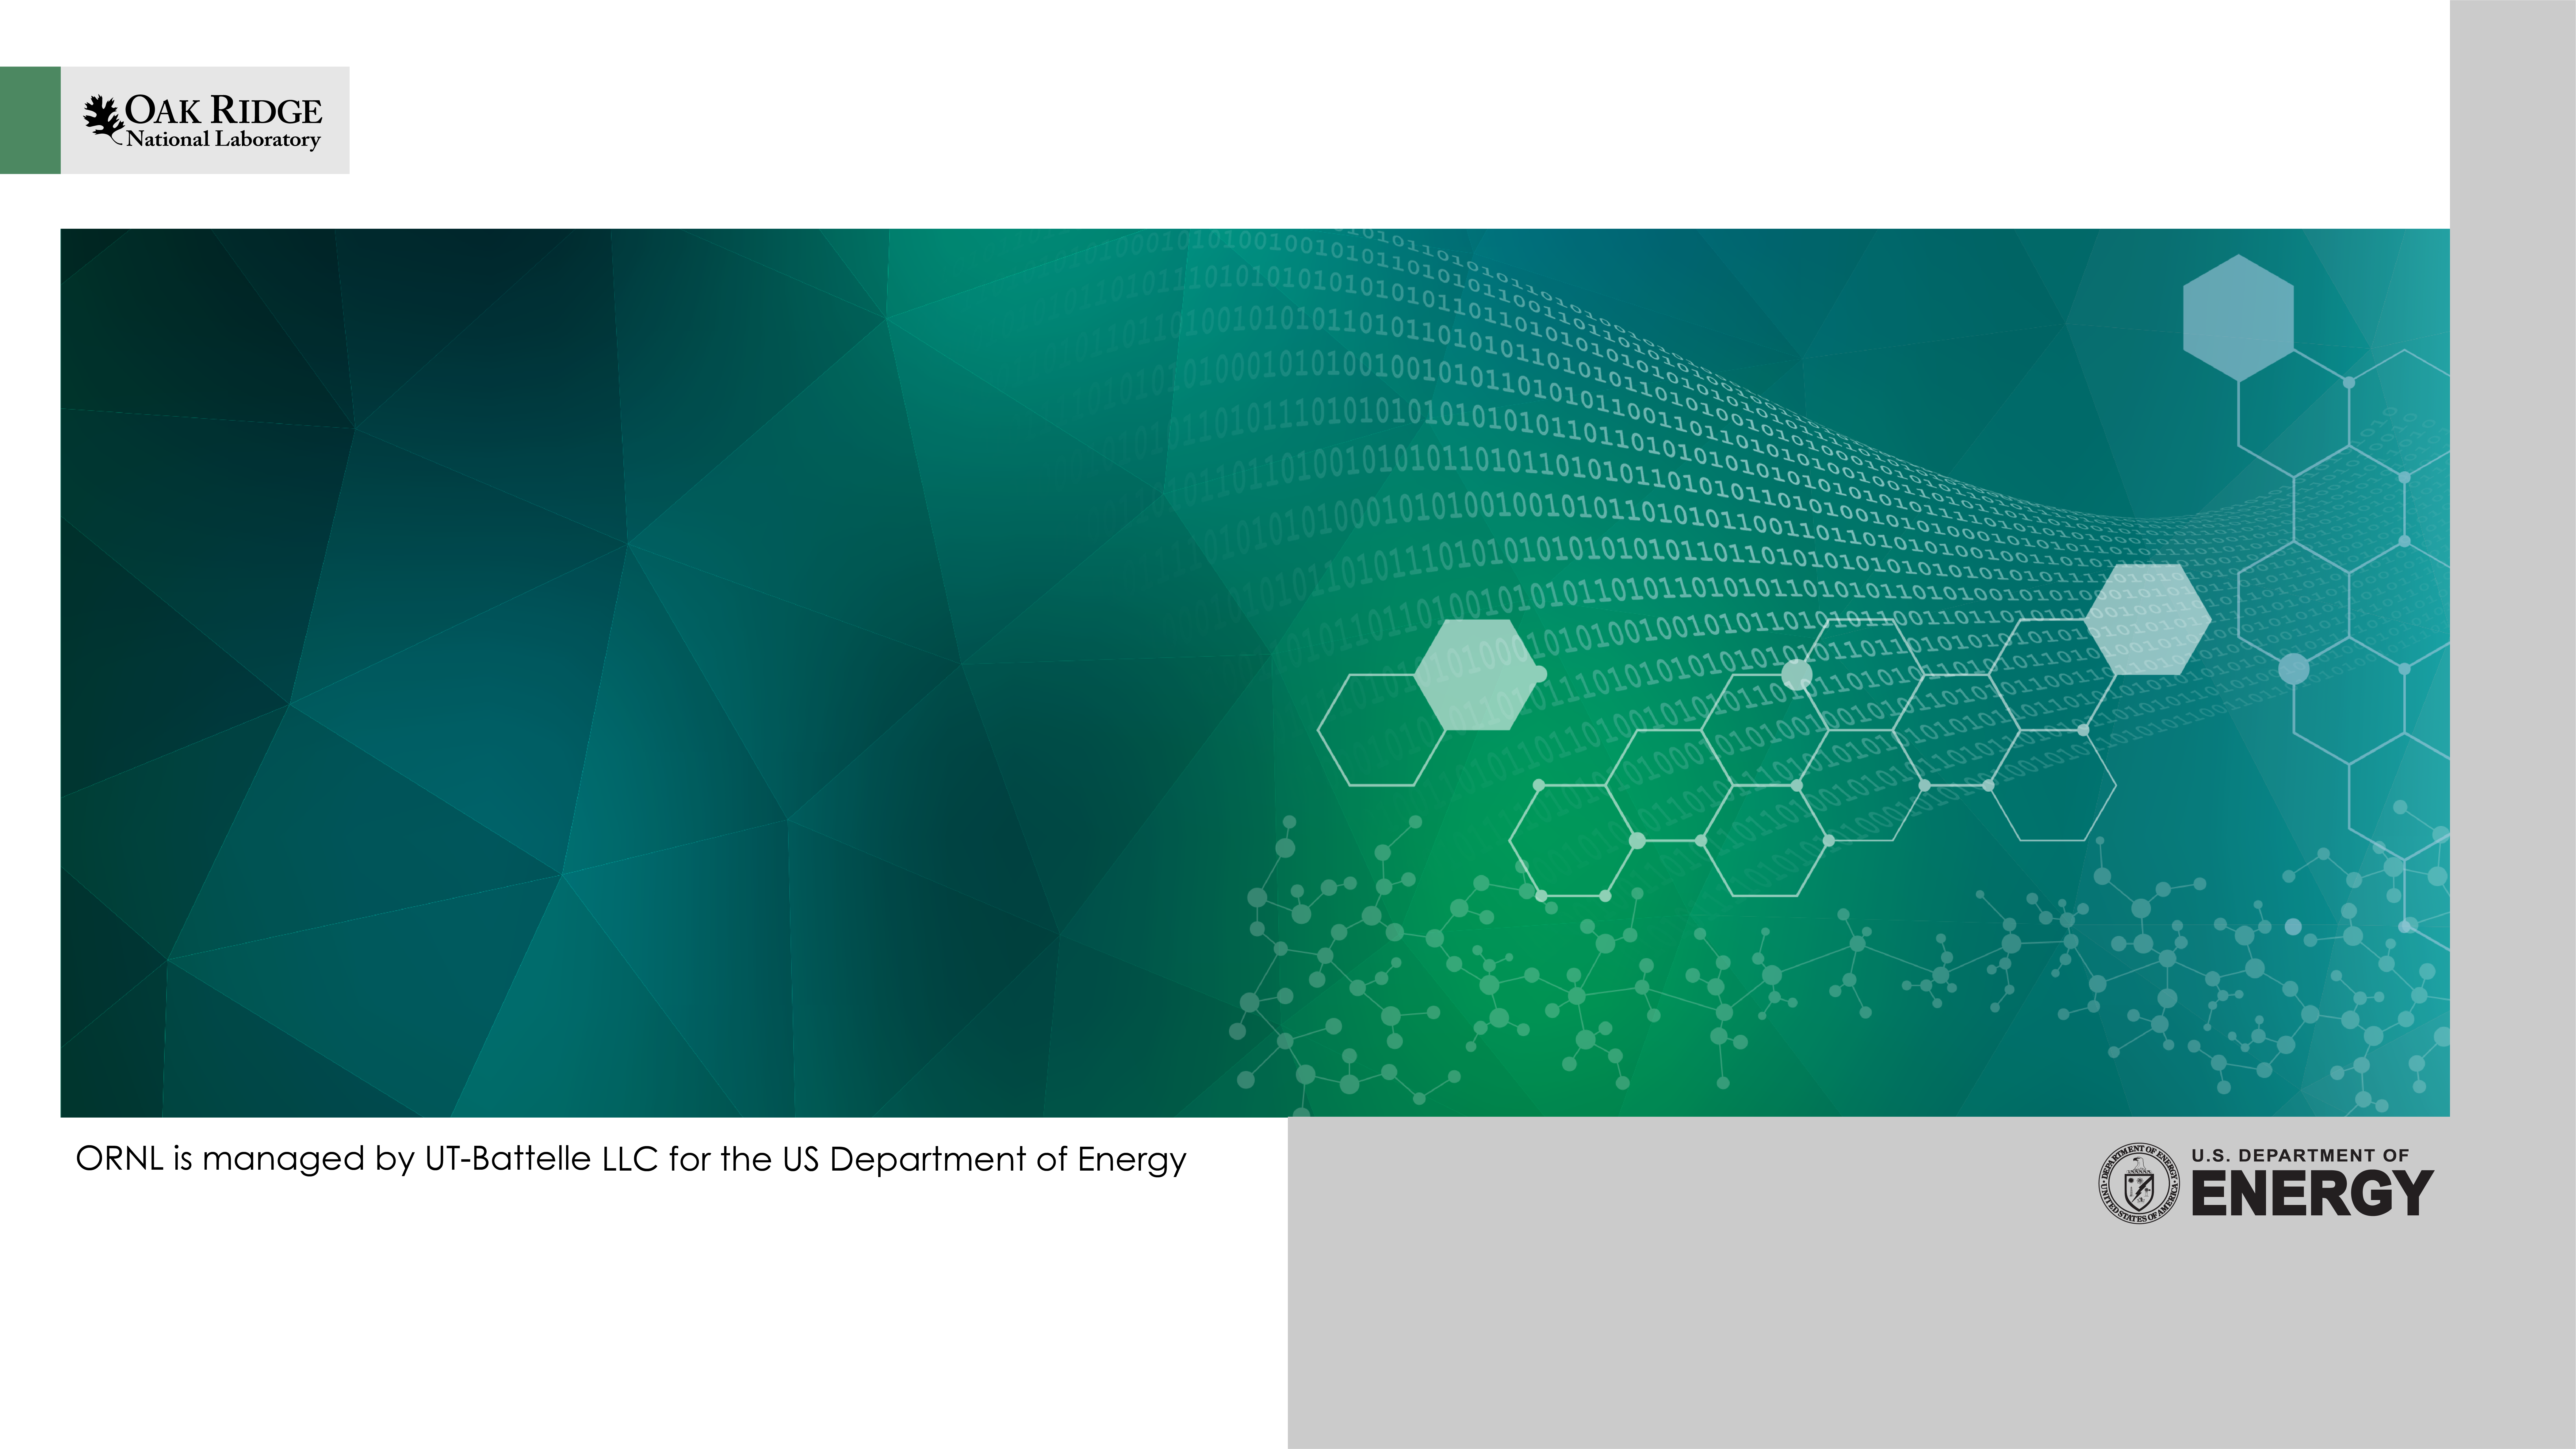
\includegraphics[angle=0,width=\paperwidth]{figs/title_frame.png}}
\setbeamertemplate{footline}{}
\begin{frame}
%%%%%%%%%%%%%%%%%%% title %%%%%%%%%%%%%%%%%%%% 
	\textcolor{white}{\Huge Literature Review}\\
	\vspace*{0.7cm}
%%%%%%%%%%%%%%%% authors name %%%%%%%%%%%%%%%%
 	\textcolor{white}{\Large Grayson Gall}\\
 	\textcolor{white}{June 12, 2023}
%%%%%%%%%%%%%%%%%%%%%%%%%%%%%%%%%%%%%%%%%%%%%%

\end{frame}
}



%
% Regular slide
%

\begin{frame}
\frametitle{\Large{Slide title}}
	\centering
	\begin{itemize}
		\item This template uses the \LaTeX~beamer package to write slides
		\item For writing mathematical equations, it is much easier to use
		\[
			\alpha\beta = \frac{dx}{dt}\gamma\Omega
		\]
		\item This template was designed by Joe Osborn and inspired by the ORNL PowerPoint template
	\end{itemize}
\end{frame}



\end{document}